\section{Proposed approach}
\label{sec:apprach}

Our objective is to extract a catalog of reusable language modules from a given set of DSLs (that we refer to as the \textit{input set}). To this end, we propose an approach based on the aforementioned notions of overlapping and potential reuse. Concretely, in our approach we first identify syntactic and semantic overlapping among the DSLs of the input set. Then, we cut such overlapping in order to break-down the DSLs in reusable language modules. Those language modules are encapsulated in such a way that they can be later composed each other in order to obtain complete DSLs. The overall strategy is illustrated in Figure \ref{fig:breakingdown}. This section is dedicated to explain it in detail.

\begin{figure}
\centering
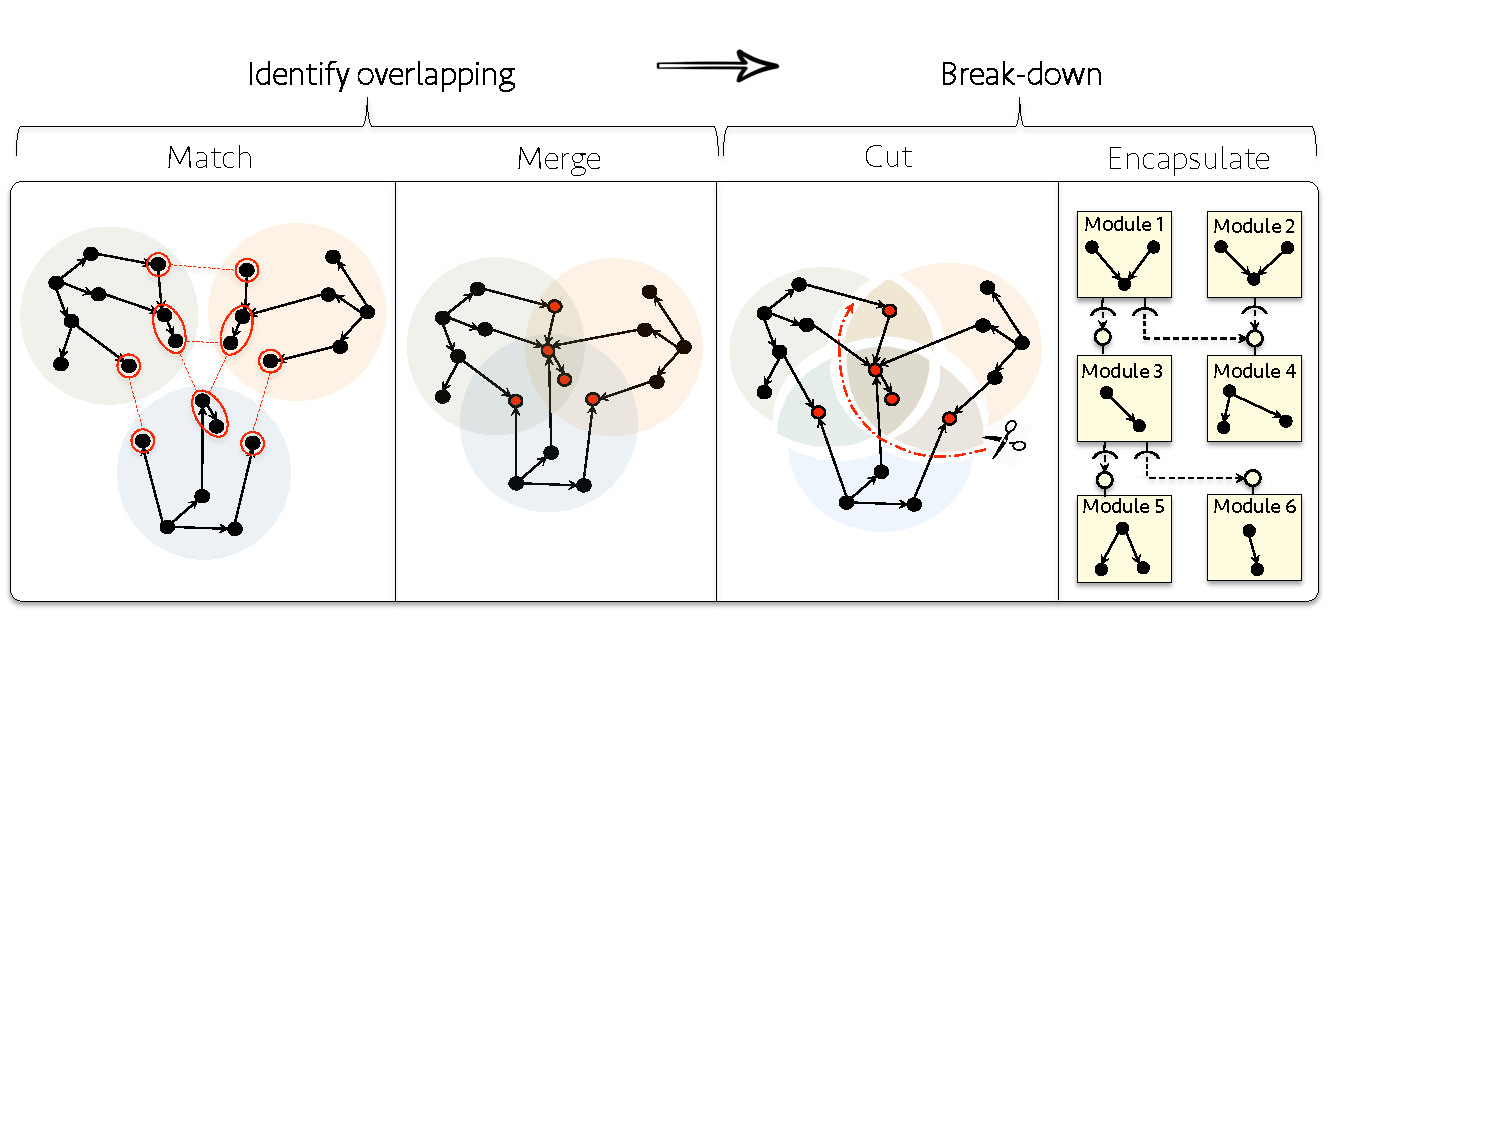
\includegraphics[width=1\linewidth]{images/breakdown.pdf}
\caption{Breaking down the input set by cutting overlapping}
\label{fig:breakingdown}
\end{figure}

\subsection{Identifying overlapping: \textit{match} and \textit{merge}}
\label{sec:identifyingoverlapping}

Our strategy to identify \textbf{syntactic overlapping} is based on the fact that a metamodel can be viewed as a direct graph where nodes represent metaclasses and arcs represent references between metaclasses. Since each DSL of the input set has a metamodel, we can represent each DSL as a directed graph. The objective now is to detect replicated nodes and organize them in the form of a Venn diagram as illustrated in the two first steps shown in Figure \ref{fig:breakingdown}.

To this end we execute a twofold algorithm. First, we perform a matching process that receives a set of metamodels (one for each DSL of the input set) and returns a set of tuples containing all the overlapping (i.e., metaclasses that are \textit{equal}) among these metamodels. Second, we merge the matched metaclasses in order to create the intersections as actual common metaclasses shared by the DSLs in the input set. For each metaclass, we store the information about what are the DSLs that use it. Note that the merging process can be viewed as a mechanism to remove repeated metaclasses.

Once the metaclasses are merged, we analyze the corresponding domain specific actions. Particularly, we check if the domain-specific actions associated to the matching metaclasses are equal as well. If so, we also have \textbf{semantic overlapping} and the merging process is extended also to the domain-specific actions. Otherwise, we create different clusters of domain-specific actions, one for each meta-class, thus establishing a \textbf{semantic variation point}. In other words, we create two different implementations of the semantics of the same metaclass that can be chosen at composition.

%\begin{equation}
%  Venn_{syn} : set(MM) \rightarrow set(<set(MM),set(MC)>)
%\end{equation}

%\begin{equation}
%  Venn_{syn}(mms) = \{<x,y> \mid x \in \mathcal{P}(mms), y = I_{syn}(x)\}
%\end{equation}

%Note that our algorithm relies on a function $I_{syn}$ that computes the intersection existing withing a given set of metamodels. It can be formalized as follows:

%\begin{equation}
%  I_{syn} : set(MM) \rightarrow set(MC)
%\end{equation}
%\vspace{-2mm}
%\begin{equation}
%  I_{syn}(mms) = \bigcap _{i=0}^{|mms|}mms_i
%\end{equation}

%Similarly, our algorithm for detecting \textbf{semantic intersections} can be described as a function that receives a set of aspects (one for each DSL of the input set) and returns a set of tuples containing all the intersections among these aspects. 

%\begin{equation}
%  Venn_{sem} : set(A) \rightarrow set(<set(A),set(DSA)>)
%\end{equation}

%\begin{equation}
%  Venn_{syn}(mms) = \{<x,y> \mid x \in \mathcal{P}(mms), y = I_{sem}(x)\}
%\end{equation}
%\vspace{2mm}

%This time, the algorithm for semantic commonalities relies on a function $I_{sem}$ that computes the intersection existing withing a given set of aspects. It can be formalized as follows:

%\begin{equation}
%  I_{sem} : set(A) \rightarrow set(DSA)
%\end{equation}
%\vspace{-2mm}
%\begin{equation}
%  I_{sem}(dsas) = \bigcap _{i=0}^{|dsas|}dsas_i
%\end{equation}

It is worth noting that detection of both syntactic and semantic overlapping relies on comparison of metaclasses and domain-specific actions respectively. At this point we need to clearly define such notion of equality that, as a matter of fact, is quite important to avoid alterations on the DSLs after the extraction of reusable language modules.

\vspace{-3mm}
\subsubsection{Comparison of metaclasses:} An operator for metaclasses comparison can be specified as follows: 

\begin{equation}
  \doteq~: MC \times MC \rightarrow bool
\end{equation}

To implement such operator, one can intuitively think that a first approach to compare meta-classes is by comparing their names. Certainly, this approach results quite useful and it is quite probable that, we can find potential reuse. For example, one can expect that in a set of DSLs for finite state machines DSL, the construct \texttt{Transition} can be considered as a commonality.

Unfortunately, comparison of metaclasses by using only their names might have some problems. There are cases in which two meta-classes with the same name are not exactly the same since they do not represent the same domain concept or because there are domains that use similar vocabulary. For instance, whereas in many cases the transitions of a state machine are only specified in terms of triggers and constraints, there are certain DSLs for state machines that allow to annotate transitions are annotated with time flags \cite{Graf:2007}.

In such cases, reuse is not that simple and a more restrictive operator should be considered. An approach that certainly helps is to compare metaclasses not only by their names but also by their attributes and references. Although this strategy can be quite restrictive, it guarantees that the detected reuse opportunities correspond to exact code clones so they can be extracted as reusable modules without any risk of altering the behavior of the DSLs. Hence, in our approach we use the later strategy. Nevertheless, we consider that certain flexibility might be to define those operators. We provide an extensible approach where other operators (such as the surveyed in \cite{Lafi:2011}) can be easily incorporated.

%\vspace{-1mm}
%\begin{equation}
%\begin{split}
%  MC_{A} \doteq MC_{B} &= true \implies \\
%   & MC_{A}.name = MC_{B}.name
% \end{split}
%\end{equation}

%\begin{equation}
%  \doteqdot~: MC \times MC \rightarrow bool
%\end{equation}
%\vspace{-1mm}
%\begin{equation}
%\begin{split}
%  MC_{A} \doteqdot MC_{B} &= true \implies \\
%   & MC_{A}.name = MC_{B}.name ~ \wedge \\
%   & \forall a_1 \in MC_{A}.attr \mid (\exists a_2 \in MC_{B}.attr \mid a_1 = a_2) ~ \wedge \\
%   & \forall r_1 \in MC_{A}.refs \mid (\exists r_2 \in MC_{B}.refs \mid r_1 = r_2)
%  \end{split}
%\end{equation}

\vspace{-3mm}
\subsubsection{Comparison of domain-specific actions:} In turn, the operator for comparison of domain-specific actions can be specified as follows:

\begin{equation}
  \circeq~: DSA \times DSA \rightarrow bool
\end{equation}

Like methods in Java,domain specific actions have a signature that specifies its contract (i.e., return type, visibility, parameters, name, and so on), and a body where the behavior is actually implemented. In that sense, the implementation of a comparison operator for domain-specific actions can be performed by checking if their signatures are equal. This approach is practical and also reflects potential reuse; one might think that the probability that two domain-specific actions with the same signatures are the same is elevated.

However, during the conduction of this research we realized that there are cases in which signatures comparison is not enough. Two domain-specific actions defined in different DSLs can perform different computations even if they have the same signatures. For example, we can found semantic variation points in the implementation of DSLs for state machines what means that the domain-specific actions are implemented differently although their signatures are the same. As a result, we only guarantee potential reuse where we compare also the bodies of the domain-specific actions. 

Note that such comparison can be arbitrary difficult. Indeed, if we try to compare  the behavior of the actions we will have to deal with the semantic equivalence problem that, indeed, is known as be undecidable \cite{Lucanu:2013}. In this case, we a conservative approach is to compare only the structure (abstract syntax tree) body of the domain-specific action (such as proposed by Biegel et al \cite{Biegel:2010}). In our approach we use the later strategy, again, in order to guarantee that semantic overlapping correspond to exact clones.

%\vspace{-1mm}
%\begin{equation}
%\begin{split}
%  DSA_{A} & \circeq DSA_{B} = true \implies \\
%   & DSA_{A}.name = DSA_{B}.name ~ \wedge \\
%   & DSA_{A}.returnType = DSA_{B}.returnType ~ \wedge \\
%   & DSA_{A}.visibility = DSA_{B}.visibility ~ \wedge \\
%   & \forall p_1 \in DSA_{A}.params \mid (\exists p_2 \in %DSA_{B}.params \mid p_1 = p_2)
% \end{split}
%\end{equation}

%\begin{equation}
%  \triangleq~: DSA \times DSA \rightarrow bool
%\end{equation}
%\vspace{-1mm}
%\begin{equation}
%\begin{split}
%  DSA_{A} & \circeq DSA_{B} = true \implies \\
%   & DSA_{A}.name = DSA_{B}.name ~ \wedge \\
%   & DSA_{A}.returnType = DSA_{B}.returnType ~ \wedge \\
%   & DSA_{A}.visibility = DSA_{B}.visibility ~ \wedge \\
%   & \forall p_1 \in DSA_{A}.params \mid (\exists p_2 \in DSA_{B}.params \mid p_1 = p_2)  ~ \wedge \\
%   & DSA_{A} \circeq DSA_{B} ~ \wedge \\
%   & DSA_{A}.AST = DSA_{B}.AST
% \end{split}
%\end{equation}


%It is worth nothing that there is this phenomenon of \textit{semantical variability}. A necessary condition to decide whether two language constructs are equivalent is that both, the metaclass and the associated domain-specific actions are equivalent. This condition guarantees that the specification is the same not only at the level of the abstract syntax but also at the level of the semantics. However, there is a phenomenon in the literature that corresponds to semantical variability \cite{Cengarle:2009}. There is semantical variability when there there are two constructs that have the same abstract syntax (i.e., their metaclasses are equal) but that differ in the domain-specific actions. This case is of interest for us because even in the presence of semantical variability we can have some potential reuse. If the metaclasses of two constructs are the same we can reuse them even if their domain-specific actions are different. 

%\vspace{-2mm}
%\subsubsection{Visualizing semantical variability:} Note that the phenomenon of semantical variability is evident in the example presented. Where there are syntactic commonalities between DSLs Logo and FSM, there are not semantic commonalities. As an additional feature of our approach, we provide a visualization of the semantical variability phenomenon. The idea is that language designers can see what are the variations in the domain specific actions.
%\todo[inline]{Usa el ejemplo para ejemplificar}

\subsection{Breaking down the input set: \textit{cut} and \textit{encapsulate}}

After being identified overlapping among the DSLs in the input set, we extract a set of reusable language modules. To this end, we adopt the idea presented by V\"oelter et al \cite[p. 60-61]{voelter:2013}: we break-down the overlapping by creating one language module for each different intersection as illustrated in the third step of Figure \ref{fig:breakingdown}. The reasoning to this solution is quite simple: by definition, an intersection is a set of language constructs that are shared by two or more DSLs. If we extract those language constructs in separated language modules, the language module can be defined once and reused by all the DSLs that require it. So, we can consider that the extracted language module is reusable. 

In our approach, we implemented this separation of overlapping as a graph partitioning algorithm. The algorithm receives the graph(s) obtained from the merging process and returns a set of node clusters: one cluster for each intersection of the Venn diagram. Arcs defined between nodes in different clusters can be considered as cross-cutting dependencies between clusters. Then, we encapsulate each nodes cluster in the form of language modules. Each module contains a metamodel, a set of domain-specific actions, and a set of dependences towards other language modules. 

Dependencies between language modules are supported by means of the classical required and provided roles in components-based software development. There is a \textit{requiring module} that uses some constructs provided by a \textit{providing module}. The requiring module has a dependency relationship towards the providing one that, in the small, is materialized by the fact that some of the classes of the requiring module have references (simple references, containment references, or inheritances) to some constructs of the providing one. In order to avoid direct references between modules, we introduce the notion of interfaces for dealing with modules' dependencies. The requiring language has a \textit{required interface} whereas the providing one has the \textit{provided interface}. A required interface contains the set of constructs required by the requiring module which are supposed to be replaced by actual construct provided by other module(s) (see Figure \ref{fig:approaches-interfaces}).

We use \textit{model types} \cite{Steel:2007} to express both required and provided interfaces. A module can have some references to the constructs declared in its required interface. In turn, the relationship between a module and its provided interface is \textit{implements} (deeply explained in \cite{Degueule:2015}). A module implements the functionality exposed in its model type. If the required interface is a subtype of the provided interface, then the provided interface fulfills the requirements declared in a required interface. 

\begin{figure}
\centering
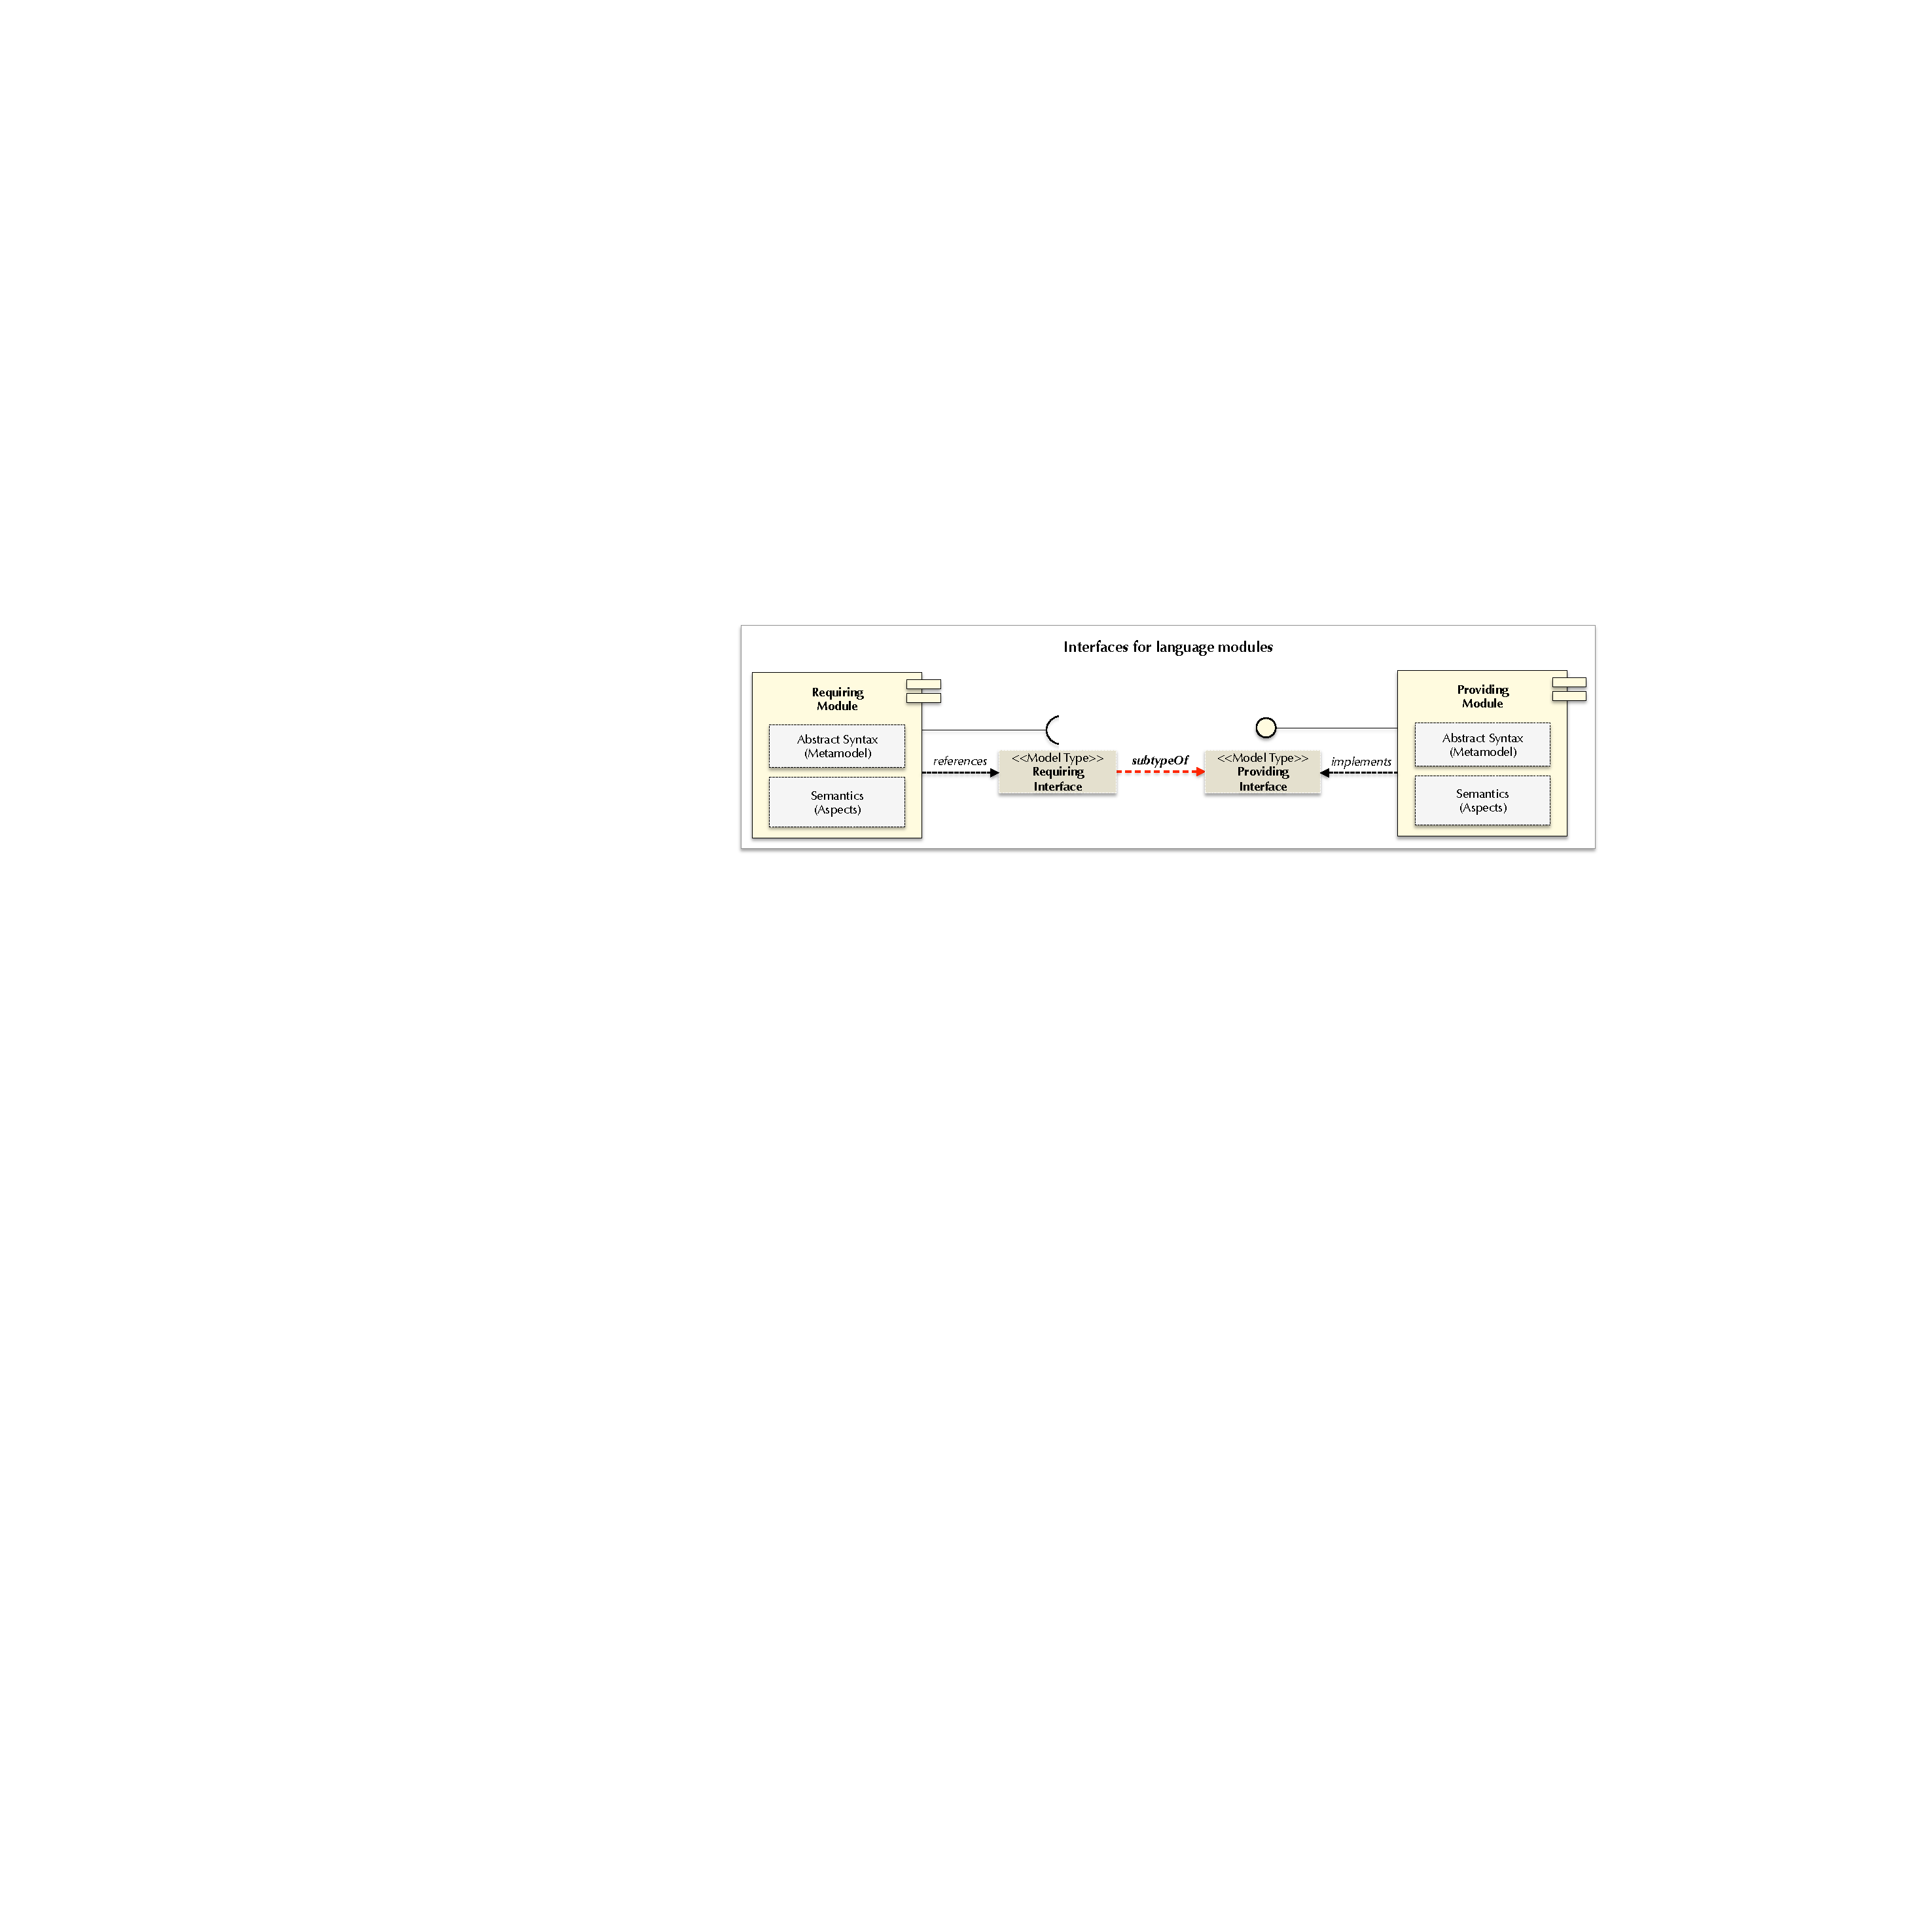
\includegraphics[width=1\linewidth]{images/approach-interfaces.pdf}
\caption{Interfaces for language modules}
\label{fig:approaches-interfaces}
\end{figure}
\vspace{-3mm}
